\documentclass[12pt]{article}
\usepackage{graphicx}
\usepackage {color}
\usepackage{pdfpages}
\usepackage{float}
\usepackage{changebar}
\usepackage{enumitem,amssymb}
\renewcommand{\familydefault}{\sfdefault}
\usepackage[margin=1.2in]{geometry}
\usepackage{graphicx}
\usepackage{wrapfig}
\usepackage[super]{cite}
\usepackage{subcaption}
\usepackage[table]{xcolor}
\usepackage{amsmath}
\usepackage[sort, numbers]{natbib}
\usepackage{multirow}
\usepackage{tabularx}
\usepackage{siunitx}
\usepackage{matlab-prettifier}
\usepackage{wrapfig,lipsum,booktabs}
%%%%%%%%%%%%Defining the margins %%%%%%%%%%%%%%%%%%%%%
\textheight 9.in
\textwidth 6.5in
\topmargin -.5in
\oddsidemargin 0in
\setlength{\parskip}{\smallskipamount}

%%%%%%%%%%%%%%Specific Commands %%%%%%%%%%%%%%%%%%
\newcommand{\eg}{{\em e.g.,}}
\newcommand{\ie}{{\em i.e.,}}
\newcommand{\etc}{{\em etc.,}}
\newcommand{\etal}{{\em et al.}}
\newcommand{\degrees}{{$^{\circ}$}}
\newcommand{\fig}[1]{\textbf{Figure #1}}

%%%%%%%%%%%%%%%%%%%%%%%%%%%% Setting to control figure placement
% These determine the rules used to place floating objects like figures 
% They are only guides, but read the manual to see the effect of each.
\renewcommand{\topfraction}{.9}
\renewcommand{\bottomfraction}{.9}
\renewcommand{\textfraction}{.1}
\renewcommand{\familydefault}{\sfdefault} %setting the san serif font

%%%%%%%%%%%%%%%%%%%%%%%% Line spacing
% Use the following command for ``double'' spacing
%\setlength{\baselineskip}{1.2\baselineskip}
% and this one for an acceptable NIH spacing of 6lpi based on 11pt
%\setlength{\baselineskip}{.9\baselineskip}
% The baselineskip does not appear to work when we include a maketitle
% command in the main file.  Something there must set the line spacing
% If we use this next command, then things seem to work.
\renewcommand{\baselinestretch}{.9}

\setcounter{secnumdepth}{0} %make no numbers but have a table of contents


\begin{document}

\title{HW 3: Medical Imaging Systems}
\author{Jake Bergquist, u6010393 }
\maketitle

\section{Q1}
\noindent\textbf{a: }
For question 1 I have re-drawn the sequence on the attached pages as can be seen in Drawing 1.  The colors used correspond to the traversal of the K space in Drawing 2. On Drawing 2 a solid line designates a sampling and a dotted line signifies a traversal of the K space without sampling. The $G_X$ axis is shown in red and the $G_Y$ axis is shown in blue. The numbers labeling the traversals of the K space on Drawing 2 correspond to the different pulses in the sequence depicted in Drawing 1. In each case all of the $G_X$ pulses are assumed to be equal (having equal area under the curve) except for the first $G_X$ pulse which is assumed to have a an area under the curve that is half that of the subsequent ones. All of the $G_Y$ pulses are assumed to have equal magnitude of area under the curve (some being negative). All traversals of the K space are thus given in a unit length. Following the trajectory from the origin first there is a dephasing pulse on $G_X$ (1) that moves us to a position in the positive direction on the $G_X$ axis of the K space to (1,0). Then there is a 180 pulse (2) that causes a traversal to a place on the negative $G_X$ axis to (-1,0). Next there is a $G_y$ pulse (3) that moves us to (-1.1) in the K space, followed by the first acquisition pulse (4) which acquires samples as we move from (-1,1) to (1,1). Next there is an inversion (5) that moves us to (-1,-1) followed by a negative $G_Y$ pulse (6) that moves us to (-1,-2). Then another acquisition(7) as we move to (-1,-2) to (1,-2). Then an inversion (8) to (-1,2). Then a positive $G_Y$ (9) to move to (-1,3). Then an acquisition (10) as we move to (1,3). Then an inversion (11) to (-1,-3). Then a negative $G_Y$ (12) to move to (-1,-4). Then the final acquisition as we move to (1,-4).

\noindent\textbf{b: } Drawing 3 shows the modifications to the sequence and the subsequent K space trajectories. In order to sample only in the positive $G_y$ area of the K space with lines like we did in part A first we allow the same $G_x$ positioning pulse (1) to move to a positive X position(1,0). Next we allow the 180 degree RF pulse to put us a (-1,0), followed by the first acquisition as we move to (1,0) again. From here there are many choices on how to use the $G_y$ to get us to a starting position where we can take another sample, preferably at (-1,1). I chose to have a negative $G_y$ pulse (4) move us to (1,-1), then the subsequent inversion (5) will move us to the desired (-1,1) where we can take the next acquisition as we move to (1,1) using a $G_x$ pulse (6). Next we need another negative $G_y$ pulse (7) with the same area under the curve as pulse 4 to move us to (1,0) before the 180 RF (8) moves us to (-1,0). Now we need a $G_y$ pulse (9) with twice the area under the curve as 4 or 7, and this time it is a positive pulse to move us to (-1,2). Following this is a $G_x$ acquisition (10) that takes us to (1,2), followed by a negative $G_y$ pulse (11) with twice the area under the curve as 4 or 7, taking us to (1,0), then a 180 flip (12) to get to (-1,0). Next we have a positive $G_y$ (13) with three times the area under the curve as 4 or 7 to get to (-1,3) and a final acquisition $G_x$ pulse (14) to get to (1,3). In contrast with the previous sequence which was able to sample the K space at successively greater distances from the origin, while maintaining the same amount of energy input to the gradients for each cycle, this sequence requires increasing energy to be provided to the $G_y$ coil in order to perform the proper K space positioning, making this sequence more difficult and costly to perform from an energy expenditure stance. Also it becomes more and more difficult to increase the area under the curve for the $G_y$ pulses without increasing the time of the pulse, which would hamper the speed of the sequence.

\section{Q2}
\noindent\textbf{a: }
Looking at sequence a it was clear that I would achieve this sort of pattern using sin and cos waveforms of the two gradients.  However simply using a sin for one gradient and a cos for the other would result in a circular trajectory in the K space when the two were integrated and used to plot the K space trajectory. Thus there needed to be a term that started at zero and constantly increased as time went on such that the amplitudes of the sin and cos functions would increase result in spirals. The easiest way to do this was to multiply the function defining the waveform by time. My initial sketch for what this should look like in the pulse sequence is shown in Drawing  4. Note that after excitation the acquisition is constant as the $G_x$ and $G_y$ change in the linearly increasing sinusoidal waveform.

The second sequence was not as easily drawn out with simple trig function. It shows a repetitive sequence of alternating directions of $G_x$ pulses interspaced with negative $G_y$ pulses to advance the sampling through the K space. There is first an initial positioning pulse on both gradients to get to the starting position. These Sequences are depicted in Drawing 5.

\noindent\textbf{b: }
The matlab code below was used to generate k-space sampling matching those presented. I had to change around the sin and cos functions for the spiral plot a few times to make sure it started in the proper position and went in the proper direction. The resulting K space sampling is shown in Figure~\ref{fig:spiral}. A shows the K space sampling resulting from the gradients shown in B and C. As for the second pattern Figure~\ref{fig:step} shows the matlab results wit A being the K space trajectory, B being the x gradient and C being the Y gradient. The red line denotes a positioning trajectory while the blue line denotes the sampling trajectory.


\begin{figure}[H]
\begin{subfigure}{\textwidth}
	
	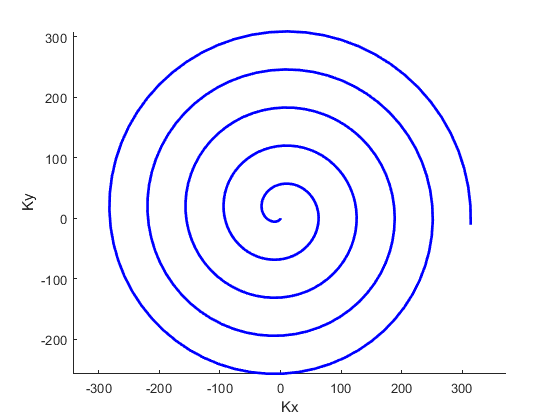
\includegraphics[width=\textwidth]{Figures/SpiralK.png}
	\caption{}
	\label{Fig:spiralK}
\end{subfigure}
\begin{subfigure}{0.5\textwidth}
	
	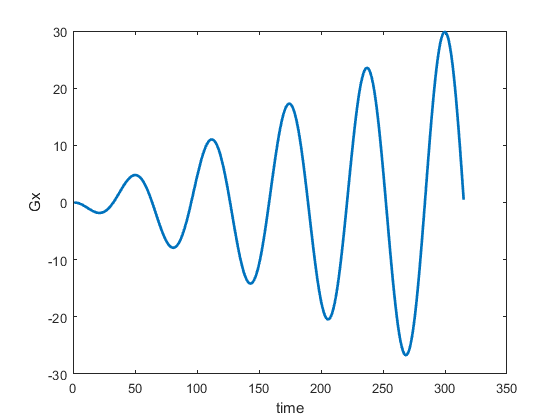
\includegraphics[width=\textwidth]{Figures/SpiralGx.png}
	\caption{}
	\label{Fig:spiralGx}
\end{subfigure}
\begin{subfigure}{0.5\textwidth}
	
	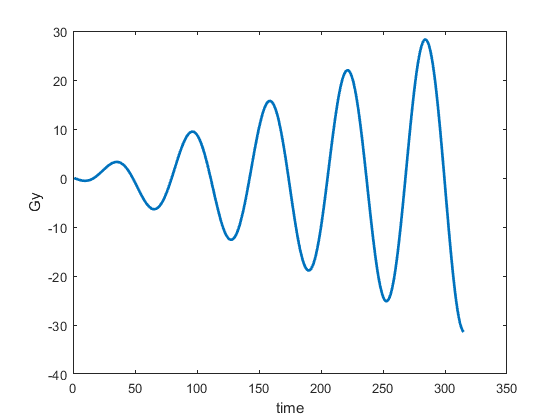
\includegraphics[width=\textwidth]{Figures/SpiralGy.png}
	\caption{}
	\label{Fig:spiralGy}
\end{subfigure}
\caption{The K space trajectory and associated gradients for the spiral pattern. A shows the rresulting trajectory. B shows the X gradient, and C shows the Y gradient. The units of the axes are 1/distance for A, and Gauss/distance squared by time for B and C. Teh actual values of the axes are irrelevant to replicating the pattern as the pattern can be scaled to match desired axes limits.}
\label{fig:spiral}
\end{figure}

\begin{figure}[H]
\begin{subfigure}{\textwidth}
	
	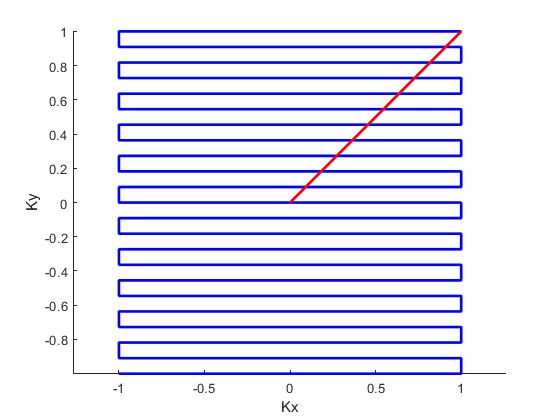
\includegraphics[width=\textwidth]{Figures/StepK.png}
	\caption{}
	\label{Fig:stepK}
\end{subfigure}
\begin{subfigure}{0.5\textwidth}
	
	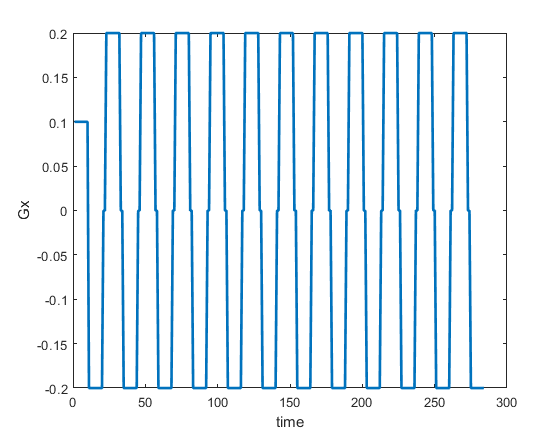
\includegraphics[width=\textwidth]{Figures/StepGx.png}
	\caption{}
	\label{Fig:stepGx}
\end{subfigure}
\begin{subfigure}{0.5\textwidth}
	
	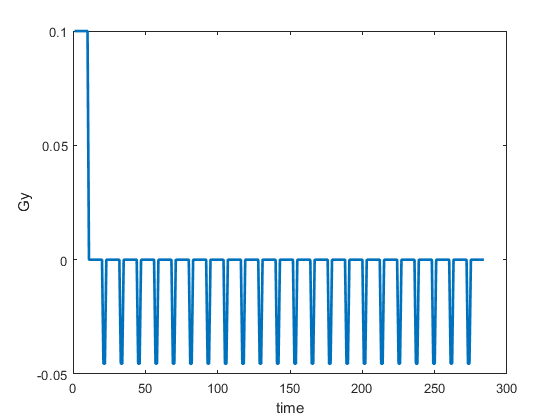
\includegraphics[width=\textwidth]{Figures/StepGy.png}
	\caption{}
	\label{Fig:stepGy}
\end{subfigure}
\caption{The K space trajectory and associated gradients for the step pattern. A shows the resulting trajectory with an initial positing in red and the sampling in blue. B shows the X gradient, and C shows the Y gradient. The units of the axes are 1/distance for A, and Gauss/distance squared by time for B and C. Teh actual values of the axes are irrelevant to replicating the pattern as the pattern can be scaled to match desired axes limits.}
\label{fig:step}
\end{figure}

\begin{lstlisting}[style=Matlab-editor]
%Q2
%part 1 making a spiral with trig functions
timeSpiral = [0:.1:10*pi];
xgradSpiral = -sin(timeSpiral).*timeSpiral;
ygradSpiral = -cos(timeSpiral).*timeSpiral;
%negative one at each time instance with a 180 flip
flipSpiral = ones(length(timeSpiral),1);
%one when sampling, 0 when positioning
sampleSprial = ones(length(timeSpiral),1);
%Function defined below
PlotKSpace(xgradSpiral,ygradSpiral,flipSpiral,sampleSprial,1);
figure(2);
plot(xgradSpiral,'linewidth',2)
xlabel('time');
ylabel('Gx');

figure(3)
plot(ygradSpiral,'linewidth',2)
xlabel('time');
ylabel('Gy');
%Part two making a start step

%get it into the starting position
clear
xgradStep(1:10) = .1;
ygradStep(1:10) = .1;

%The following segments will be repeated to do each step
repeatXgrad(1:10) = -.2;%First going backwayrds in x
repeatYgrad(1:10) = 0;%And not moving on y
%There are 11 steps to go from the most positive y value to the y axis, and
%I assume a unit value for the maximum y. Let's assume we only take two
%time steps to get from one y level to another
repeatXgrad(11:12) = 0;%Don't move x during this time
repeatYgrad(11:12) = -1/22;%11 steps per 1 unit, but pbroken into two steps makes 22 per one unit

repeatXgrad(13:22) = .2;%now go forward in x
repeatYgrad(1:10) = 0;%And not moving on y

repeatXgrad(23:24) = 0;%Don't move x during this time
repeatYgrad(23:24) = -1/22;%11 steps per 1 unit, but pbroken into two steps makes 22 per one unit

%Repeat the above 11 times then add one final negative x move

addOnX = repmat(repeatXgrad,1,11);
addOnY = repmat(repeatYgrad,1,11);

xgradStep = [xgradStep,addOnX,-.2.*ones(1,10)];
ygradStep = [ygradStep,addOnY,zeros(1,10)];

samplingStep = ones(length(xgradStep),1);
samplingStep(1:10)=0;

PlotKSpace(xgradStep,ygradStep,ones(size(xgradStep)),samplingStep,4);
figure(5);
plot(xgradStep,'linewidth',2)
xlabel('time');
ylabel('Gx');
figure(6)
plot(ygradStep,'linewidth',2)
xlabel('time');
ylabel('Gy');

function PlotKSpace(xgrad,ygrad,flips,sampling,figNum)
%Plots the K space trajectory. Designed with single shot trajectories in
%mind. Currently does not handle multiple positing trajectories. Assumes
%last positing location is beginning of sampling trajectory
if sampling(1) == 1
sampling = [1;sampling];
else
sampling = [0;sampling];
end

fullPath = zeros(2,length(xgrad) + 1);

for t = 1:length(xgrad)
fullPath(:,t+1) = fullPath(:,t).*flips(t);%If there is a flip at this time point, then flip the previous coordinates

fullPath(:,t+1) = fullPath(:,t) + [xgrad(t);ygrad(t)];
end
figure(figNum);clf;hold on;
%plot any positiing
%Note for future: add functionality to split
%positining paths so that they can be plotted properly if there
%Is more than one.
%Plot the sampling trajectory and positining
plot(fullPath(1,:),fullPath(2,:),'b','linewidth',2)
%Plot the positing trajectory over the sampling in a different color
plot(fullPath(1,sampling == 0),fullPath(2,sampling == 0),'r','linewidth',2)
axis('equal')
xlabel('Kx');
ylabel('Ky');
hold off

end
\end{lstlisting}

\section{Q3}
\noindent\textbf{a: }
For this problem we want to use EQ~\ref{eq1} to calculate gsl. First we solve for $G_Z$, which we can rearrange for as shown in Eq~\ref{eq2}. We choose a $\gamma$ value for hydrogen atoms in water at $42.58 \frac{MHz}{T}$ which converts to $4258 \frac{Hz}{Gauss}$. In our case the slice thickness is 1.0 mm, or 0.1 cm, which is our value for $z$. The sinc pulse for this gls1  is 4 ms, which equates to a $f_0$ of $1/4ms = 250 Hz$. Plugging in all of these number to Eq~\ref{eq2} gives us $3.69 Gauss/cm$ for Gsl1. The gsrf should have the same area under the curve as half of the gsl. If we can assume that the gsrf has a duration of half that of the gsl1 (which appears to be the case based on the image) then the amplitude of the gsrf is $-3.69 Gauss/cm$. For gsl2 the sinc pulse is twice as long, leading to a $f_0$ that is half that of gsl1, thus the aplitude of gsl2 is half that of gsl1, which is $1.85 Gauss/cm$.

\begin{equation}
f_0 = \frac{\gamma}{2\pi}G_zz
\label{eq1}
\end{equation}
\begin{equation}
G_z = \frac{2\pi f_0}{\gamma z}
\label{eq2}
\end{equation}

\noindent\textbf{b: }
For this problem we want to focus on Eq~\ref{eq3}. A similar formula holds for the $G_y$ and $K_y$ relationship. We know that the spatial frequency k space trajectory traversed ($K_x$) is equal to the inverse of the spatial domain, therefore $K_x = \frac{1}{20cm}$. Given that we want to take 192 samples (to get our 192 x 192 image) and we are working with a 50 KHz digitizer we can determine that the time of the gro pulse must be $\frac{192}{50KHz} = 0.0038 s = t$. Now given that we have rectangular pulses, and an integral calculates the area underr the curve, we can simplify Eq~\ref{eq3} by incorporating the fact that $\int_{0}^{t}G_x(\tau)d\tau = G_xt$, while also solving for $G_x$ to get Eq~\ref{eq4}. Now using the same gamma as above ($4258 Hz/Gauss$) we can plug in our known quantities and get that the gro pulse must have an amplitude of $0.019 Gauss/cm$. This corresponds to a traversal across the K space whereas given the structure of this pulse sequence, the grdp must dephase the signal into the positive X direction of th eK space before the 180 inversion sets the K space location to be at the beginning of the gro trajectory. Thus the grdp should have a duration half that of the gro and an amplitude \textbf{the same} as the gro. 

\begin{equation}
K_x = \frac{\gamma}{2\pi} \int_{0}^{t}G_x(\tau)d\tau
\label{eq3}
\end{equation}
\begin{equation}
G_x = \frac{2\pi K_x}{\gamma t}
\label{eq4}
\end{equation}

\noindent\textbf{c: }
For this part we use the same relationship established in Eq~\ref{eq4} but using terms specific for $G_y$ and $K_y$. In this case the trajectory traversed by $K_y$ totals to again be $1/20cm$ however it is broken up into 192 steps as each $G_y$ pulse only dephases us one step in either the positive or negative $K_y$ directions. Thus $K_y = \frac{\frac{1}{20 cm}}{192}$ Based on the diagram I assume that the $G_y$ gpe pulses have a duration that matches the grdp which is half of that of the gro as defined in part b. Thus using these changes we can calculate that the incremental phase encoding amplitude is $0.0002 Gauss/cm$. The initial amplitude is zero as we want at least one trajectory to traverse the origin of the k space.
	

\section{Q4}
\noindent\textbf{a: }
The required sketch is shown in Drawing 6.

\noindent\textbf{b: }
For the original sequence we know that the time between the center fo the two rf pulses is equal to half of the TE. The time in between the middle of the second RF pulse and the middle of the gro sequence is also equal to half the TE. The first pulse has a total time of 4 ms, and the second is 8 ms, thus the times between the center of the pulses and the begennings or ends are 2 and 4 ms respectivly. We know that the gro pulse, using the described digitizer, has a duration of 0.0038 sec or 3.8 ms. Thus time time between the intiaition of this pulse and its halfway point is 1.9 ms, which is also the time of the gpe and grdp pulses. the gsl pulse is 2 ms (half the duration of the gls pulse). Thus the closest the two rf pulses could get to each other (thus the shortest TE ) in this case is dictated by the widest pulse that has to be included, which in this case is the gsl at 2 ms, thus the minimal TE is 2x(2ms + 2ms + 4ms) = 16 ms. It is true that the gro could come closer to the gsl2 pulse but this would force the two slice selection gradients too close to allow for the gsrf to occur without overlap. If the gsrf could be shortened (by increasing its amplitude) to match the gpe and grdp pulses this could decrease the minimal TE to (2x(2ms+1.9ms+4ms)) 15.8ms.

For the altered pulse sequence all of the same pulse widths apply. The two pulses can only get so close as to not cause overlab between the gls pulses and the gsrf pulse. These cause a minimal again of 16 ms (2x(2+2+4)). Considering the new position of the grdp pulse this means the teoretical limit of how close in time the center of the second RF pulse and the center of the gro pulse can get goes from 5.9 ms(5 ms from the pulse, 1.9 from half of the gro) to 7.8 ms (4 ms from the rf pulse, 1.9 ms from the grdp, 1.9 ms from the gro). This however is still a shorter time that the minimum time between the two rf pulses as dictated by their widths and the width of the gsl (2ms from rf pulse 1, 2ms from gsl, 4ms from rf pulse 2). This timing of 8 ms is larger and thus the limiting factor.

\noindent\textbf{c: }
The dephase pulse being closer to the readout pulse in beneficial in the altered sequence because the signal is less influenced by noise or $T_s^*$ decay between the dephase and the readout. Additionally, there could potentially be errors associated with the 180 degree pulse that place us in a place int he K space that is not exactly where we expect it to be if we are to do the dephase before the 180 degree pulse. However if we do not dephase before the 180 pulse, any inconsistencies int he 180 pulse will not affect our K space (along the Kx axis). Additionally given the same parameters for a sequence (gro, grdp, gpe, etc) there will be a longer TE for the modified sequence. This may seem detrimental but it also allows for wider RF pulses and slice selection gradients, as there is more time to fit these longer pulses in. This allows for a bit more flexibility in the slice selection and RF pulses. Thus for a given desired flip angle, the magnitude of $G_z$ can be less.

\section{Q5}
\noindent\textbf{a: }
By plugging in the maximum gradient amplitude and solving for the time we can figure out how short we are able to get the gsrf, and grdp, and gpe. However the digitizer we are using is the same, and we want to get the same resolution image. Thus the gro cannot be any shorter. Additionally we are not changing our sinc pulses thus the gsl1 and gsl2 also cannot get any shorter. We know that the gsrf has to have the same area under he curve as half of the gsl1 pulse. The gsl1 pulse has an amplitude of 3.6 Gauss/cm as determined in question 3. We know that the gsl1 is on for 4 ms (length of the first rf pulse) thus the area under half of this pulse is 2*3.69 Gauss/cm. Thus if we use our maximum gradient amplitude we can solve for the new time. $time = (3.69x2)/4 = 1.85 ms$. We can apply the same principle to calculate the new times for the grdp and gpe pulses, however a quick look shows that these pulses will fit within the gsrf (for the grdp we get 0.0045 ms). Thus these short times do not really affect our calculation of the minimum TE. Thus the minimum TE as determined by the fact that the TE is equal to twice the time between the centers of the two sin pulses, can be determined by adding up the times for each of the halves of the ainc pulses plus the gsrf that must fit between them then multiplying by 2, which is in this case 2(2ms + 1.85ms + 4ms) = 15.7 ms. Just to check that the gro is going to fit in the time window such that the center of the gro is at the TE, thus the center of the GRO must be a half TE time past the center of the second sinc pulse: we know that using htis digitizer the gro must be 3.8ms (Q3) and the second sinc pulse has a duration of 8 ms. At a TE of 15.7 ms we know that the center of the sinc pulse and the center of the gro pulse must be 7.85 ms apart. Given these things it is clear that this is possible because the sinc pulse center and the gro center are able to be 5.9ms separated without overlapping. Thus they will fit given this TE. Note that this minimal TE is mainly determined by the gsrf, which already had an amplitude near our new maximum when we calculated it in Q3. We either need a newer gradient, or smaller sinc pulses such that we can get a shorter TE.

\noindent\textbf{b: }
For this sectoion we simply perform a manipulation of Eq~\ref{eq1} by instead solving for the z and plugging in all of the same known quantities from equation 3 with the addition of using the maximum allowed gradient amplotude of 4 gauss/cm. This gives us a slice thicknes of 0.092 cm.

Now we can look at the xy resolution inplane. Again we perform the same kind of rearrangement, this time to Eq~\ref{eq3} solving for $K_x$ bu plugging in the maximum $G_x$ of 4 Gauss/cm. We know that the spatial X traveresed is equal to $\frac{1}{K_x}$. This gives us a traversal of 0.077 cm. This is how far we scan for the entire gro, and thus the size of the assumed-to-be-square pixels is 0.097cm/192 = $5.06\mu m$ for a 192x192 pixel slice.

\end{document}



\begin{figure}[H]
	\centering
	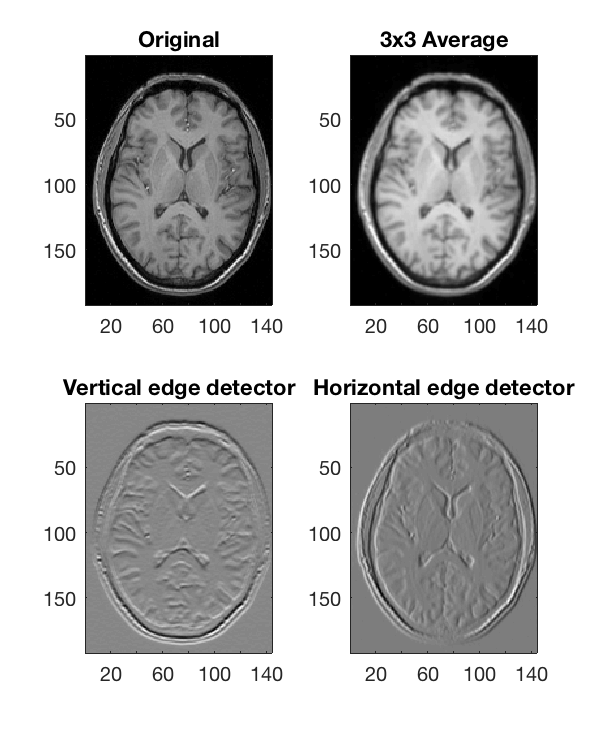
\includegraphics[width=\textwidth]{Figures/convs.png}
	\caption{}
	\label{Fig:conv}
\end{figure}






